% IN THIS SECTION SHOW SOME OF OUR TRANSLATED CODE... AND WALK THROUGH IT THE SAME WAY YOU DID WITH THE CONCEPT IN RESOLVE. BUT BEFORE YOU DO THAT, SHOW THE PICTURE (The one thats already here showing high level relationships and update it!).
\section{Implementation}
Development of our C translation tool can be logically partitioned into three distinct phases: 
\begin{enumerate}
\item Arriving at a translation model (or, strategy) for an accurate C representation of RESOLVE.
\item Implementing reusable mechanisms for carrying out the C code generation process.
\item Creation of a memory manager capable of safely allocating and freeing dynamic memory required by the generated code.
\end{enumerate}
We illustrate each of these phases working in tandem on the LED component discussed in Section \ref{sec:specifiying}. 

%In this section we discuss each of these phases using the LED component developed in Section \ref{sec:specifiying}.

\subsection{C Translation Model}
One of the primary challenges in translating from RESOLVE to C is finding a suitable C analog for each RESOLVE module and the constructs allowable in each. Indeed, since we are dealing with an environment where functional correctness is a primary concern, it is important that the code generated by our tool represents as closely as possible the original RESOLVE source. In an effort to make such considerations, at the highest level, the C code we generate makes special considerations for facilities, concepts, and realizations. 

\begin{figure}
\begin{center}
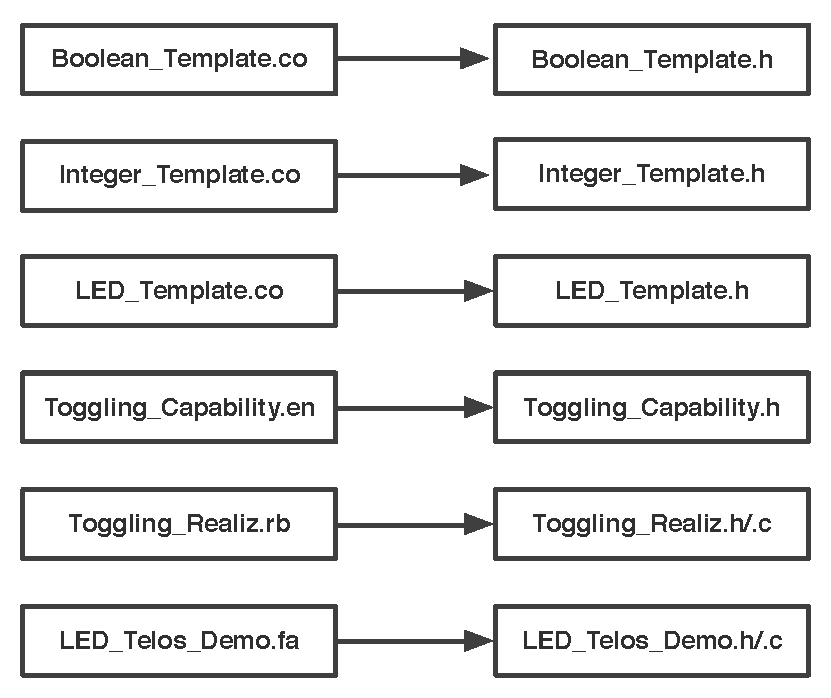
\includegraphics[scale=.55]{figs/relationship.pdf}
\end{center}
\caption{Relationship between RESOLVE module types and the C code generated from each.}
\label{fig:relationship}
\end{figure}

\subsubsection{Concepts}
Concepts produce a single .h that provide function pointers for each operation specified by the original concept, as well as structs for each user defined type. 

\subsubsection{Facilities}
Facilities produce an .h/.c pair: The header .h declares methods that are intended to manage the creation and destruction of all global variables used within the facility, while the .c provides an implementation of these methods.  Note that the create and destroy methods are only responsible for freeing \textit{global} variables, all other translated, local functions are responsible for deallocating their own variables. 

\subsubsection{Realizations}
We treat realizations of concepts and enhancements slightly different than facility modules. While a .h/.c pair is still produced, the create method for realizations is designed to create instances of all types specified by the concept, while the destroy method deallocates these types.

%The .h/.c pair generated for realizations include

%While facilities, concept realizations, and enhancement realizations in general produce an .h/.c pair, the .h produced for facility modules differs slightly from the others: Whereas realizations of concepts and enhancements provide 

% concept realizations provides methods for creating and destroying a single instance of the type declared by the concept it realizes. However, header files for realizations of facility modules provide methods creating and destroying all global variables within the facility. Common global variables include the set of standard facilities provided to every module in addition to any locally defined within the scope of the facility.
 
% responsible for declaring functions that create and destroy the objects used

%The memory model must also be considered as an additional verifiable component. Currently, RESOLVE is not capable of creating a complete specification of memory\footnote{RESOLVE is an object based language and has variable sized structures. Using dynamically allocatable memory is the favored approach to allow arbitrarily sized data.}. Thus, a memory model must be realized without a specification. To provide a straight forward translation from RESOLVE to C, we provide a dynamically-based memory allocator for use on embedded systems.



%Unsurprisingly, concepts are represented in C by a single header .h listing the various methods 

\subsection{Translator Implementation}

Translation itself is performed over the course of a traversal of RESOLVE's abstract syntax tree (AST). The traversal mechanism used is a derivative of the visitor patter that provides a pre post traversal over all nodes in the tree. 

%\subsubsection{AST Traversal}
%Translation is performed over the course of a traversal of RESOLVE's abstract syntax tree (AST). The traversal mechanism used is a dervivative of the visitor pattern that provides a SAX-dom style pre-post traversal over all nodes in the tree. Thus, for any given node present, a total of two visits occur: One corresponding to the node being `hit' during the pre traversal stage, and one for the post. 

%To make this more concrete, consider the following dummy operation.

%\begin{verbatim}
%Operation Nothing(); Procedure
%        Var X : Integer;
%        X := 3;
%end Nothing;
%\end{verbatim}

%Shown in Figure \ref{fig:ast} is the AST representation of operation \texttt{Nothing}. Here, language constructs are represented as labeled boxes, while the actual traversal over these constructs -- and the order in which it is performed -- is communicated on the right via the call stack. Each of these calls are received in the translator in the order in which they are visited within the tree. It is up to the client (in this case, the author of the C-translator) to decide which of these methods they wish to override and perform custom actions within. 

%We feel this particular traversal pattern lends itself to task of source to source translation for the following reasons:

%\begin{itemize}
%\item A visit method for a construct provides a convenient encapsulation of all the logic required to translate RESOLVE construct $x$ to appropriate C construct $y$.

%\item Overriden visit methods apply to every instance of a construct -- meaning RESOLVE's C translator requires few (if any) loops, as the walk itself serves as the method of iteration.

%\item Finally, only the visit methods for the constructs we currently wish to process need to be overridden. This makes it easy to tweak and optimize the size of the translator's codebase, implementing only visit method for language constructs that explicitly require translation.  
%\end{itemize}

%\subsubsection{Translation output}
%Output of translated code is done using \textit{Stringtemplate} -- a third-party tool written in Java that allows users to define parameterizable templates. Like the name suggests, a template is simply ``a document with holes" that the user choses when and how to fill. 

%An example C function definition template is shown below.

%\begin{verbatim}
%function_def(modifier, type, name, params, 
%                               vars, stmts) ::= <<
%<modifier> <type> <name> (<params; sep = ", ">) {
%    <vars; sep = "\n">
%    <stmts; sep = "\n">
%}>>
%\end{verbatim}

%User supplied attributes, enclosed in \texttt{<..>}, indicates the position of that attribute relative to others. It is entirely up to the user to define which attributes to fill in, and how complex they want them to be. For example, the user might choose to fill the \texttt{params} attribute with a simple string, or a separately defined \texttt{parameter} template, which in turn might use another separately defined \texttt{type} template.

%\begin{verbatim}
%parameter(type, name) ::= "<type> <name>"
%\end{verbatim}

%In the context of language translation, these templates, when stored on a stack and manipulated over the course of the aforementioned AST traversal, help simplify the task of producing complicated, structured blocks of C output. For instance, upon visiting \texttt{preOperationDec}, a \texttt{function\_def} template can be instantiated by the client and pushed onto a global translation stack with its \texttt{name}, return \texttt{type}, and \texttt{modifier} attributes filled in. As \texttt{preOperationDec}'s children are visited, the \texttt{function\_def} template currently at the top of the stack receives similarly constructed parameter, variable, and statement templates from the nodes being walked. Upon reaching \texttt{postOperationDec}, we can be assured that the function has been completely filled in with the appropriate templates -- assuming the user has implemented the children's visit methods.

%Hence, the only actual work being performed within visit methods is forwarding appropriate information from tree-node it represents, to an externally defined template. This allows us to exploit (in shameless design pattern parlance) a strict model view controller (MVC) separation in the translator's codebase between the mechanism that does the AST visiting (controller), the tree nodes from which we're adding information to templates (model), and the external file containing all available C language templates (view).

%One of the primary allures of this approach to translation is that that adheres to strict MVC design principles -- meaning that all output logic is distinctly separated from translation related logic. 

%We take advantage of these pre post methods using templates and simple stack to implement 


%Going even further, we demonstrate this by showing the steps taken to translate a simple operation declaration \texttt{nothing} to C.

% for each construct to remain encapsulated within that method, and (almost) completely eliminates the need for complex loop or iteration mechanisms. 


%This particular traversal pattern lends itself well to the language translation challenge (specifically source to source) where the pre methods align naturally with beginning of a construct, and conclude with its corresponding post method.  For instance, in the case above, this allows us, upon receiving a callback for In an effort to keep logic implementing our translator distinct and separate from the output language, we used a model view controller framework for implementing 

%To illustrate this, consider once again facility \texttt{DoNothing}.

%%%%%%%%%%%%%%%%%%%%%%%
%           Memory Allocation Section              %
%%%%%%%%%%%%%%%%%%%%%%%
\subsection{Memory Allocation}\label{sec:mem}

Memory limitations on embedded hardware has made dynamic memory allocation a difficult, or impossible practice. Many existing programs, including RESOLVE, however,  inherently use heap-based memory. Previous attempts at a RESOLVE to C translation required a constant size for each variable declaration\cite{regula:2010}. This approach can provide efficient use of memory for embedded systems, it does not, however, provide a straight forward approach to translation. In this section, we introduce a RESOLVE wrapped dynamic memory allocator implemented on the stack.

\subsubsection{Allocation using \texttt{salloc}}

The function \texttt{salloc()}, uses a first fit approach for allocation on the stack, rather than conventional, heap-based allocators. This approach requires that a fixed size of memory is chosen at compilation. In addition, \texttt{salloc()}, requires a section of meta-data, which is denoted as a \texttt{block}, for each record in the memory pool. A \texttt{block} holds referential information of neighboring blocks, the size of the record the block maintains, and if the block is free or is in use. Figure~\ref{fig:stack} is an example of the stack after several calls to \texttt{salloc()}.

\begin{figure}[!htb]
%\centering
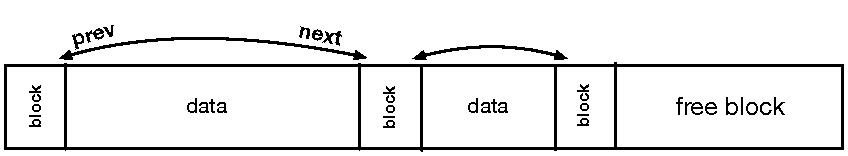
\includegraphics[scale=.55]{figs/stack.pdf}
\caption{Representation of memory using salloc()}
Memory allocated with salloc() allocates a block in front of data allocated. Blocks point to their immediate neighbors and hold their size and usage.
\label{fig:stack}
\end{figure}

\subsubsection{Deallocation using \texttt{sfree}}

A memory allocator must provide a mechanism to release, or free memory in order to indicate that it is not being used and can be reallocated. The \texttt{sfree()} function provides deallocation for memory allocated with \texttt{salloc()}. Figure~\ref{fig:free} shows an example set of memory before and after calling \texttt{sfree()}. 

\begin{figure}[!htb]
%\centering
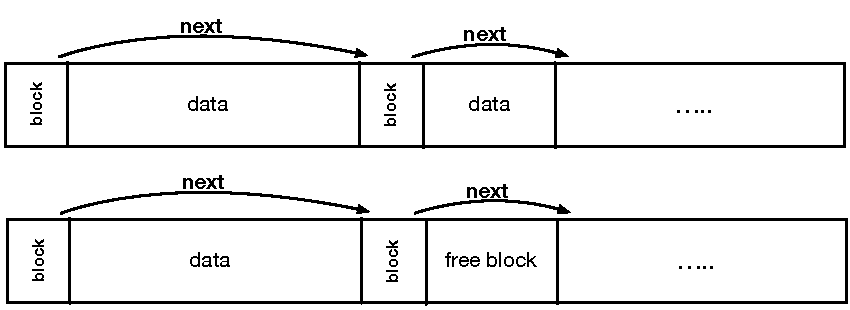
\includegraphics[scale=.55]{figs/sfree.pdf}
\caption{sfree to free memory}
\label{fig:free}
\end{figure}

\subsubsection{Optimizing Memory Usage}

A common problem that can occur in memory allocation is fragmentation. During execution, a program can allocate and deallocate an arbitrary number of times. Figure~\ref{fig:fragmentation} shows problems that result from this. This problem is magnified on embedded systems due to their limited memory capacities. There are simple optimizations that can reduce fragmentation. 

Block splitting, as shown in Figure~\ref{fig:split}, occurs during allocation. It allows blocks of greater size to be partitioned into the size requested by the allocator. 

Fusing blocks is another technique used when \texttt{sfree()} is called. When memory is deallocated, neighboring free blocks are coalesced to form a single large block, as shown in Figure~\ref{fig:fuse}. 

\begin{figure}[!htb]
%\centering
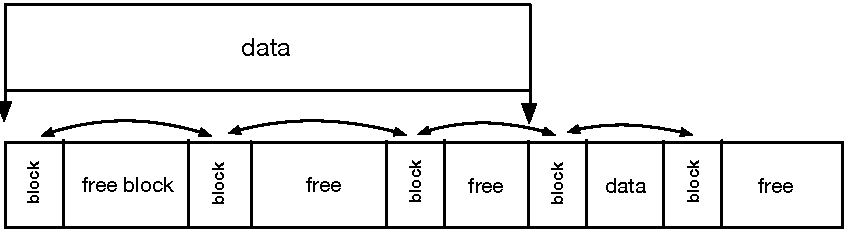
\includegraphics[scale=.55]{figs/fragmentation.pdf}
\caption{fragmentation}
\label{fig:fragmentation}
Performing many naive allocation and deallocations, allocatable blocks are restricted to those that match the exact size of memory requested from the allocator.
\end{figure}

\begin{figure}[!htb]
%\centering
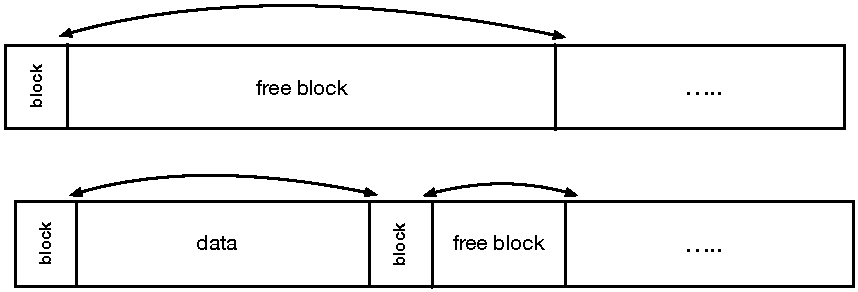
\includegraphics[scale=.55]{figs/split.pdf}
\caption{block splitting}
Splitting of a free block creates two new blocks: a block that is the size that the allocator requested, and the other contains the remainder of a new free block with the remainder of memory.
\label{fig:split}
\end{figure}


\begin{figure}[!htb]
%\centering
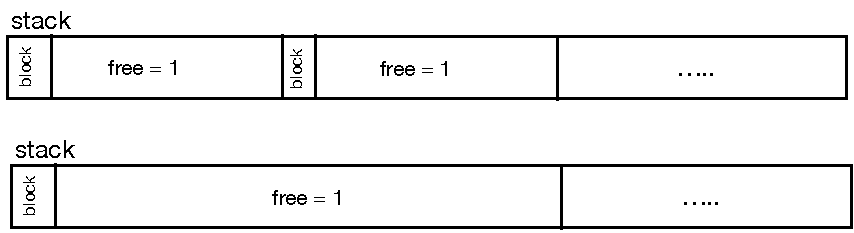
\includegraphics[scale=.55]{figs/fuse.pdf}
\caption{block fusing}
An example of fusing blocks together. This creates single larger block, decreasing the number of smaller blocks unable to split.
\label{fig:fuse}
\end{figure}

%
%